
%%%%%%%%%%%%%%%%%%%%%%%%%%%%%%%%%%%%%%%%%%%%%%%%%%%%%%%%%%%%%%%%%%%%%%%%%
% documentclass option: pick one:
% "presentation" for powerpoint-like talk,
% "handout" for  printing,
% "trans" for printing onto transparencies
%%%%%%%%%%%%%%%%%%%%%%%%%%%%%%%%%%%%%%%%%%%%%%%%%%%%%%%%%%%%%%%%%%%%%%%%%

%\documentclass[leqno,presentation]{beamer}
%\documentclass[leqno, handout]{beamer}
%\documentclass[leqno,trans]{beamer}
\documentclass[leqno,presentation,unknownkeysallowed]{beamer}

% load standard packages
\usepackage[utf8]{inputenc}
\usepackage{mathtools}
\usepackage{amsfonts}
\usepackage{amsmath,amssymb,latexsym}
\usepackage[english]{babel}
\usepackage{tikz}
\usepackage{hyperref}
\usepackage{fancyvrb}

% ######## ##     ## ######## ##     ## ########  ######
%    ##    ##     ## ##       ###   ### ##       ##    ##
%    ##    ##     ## ##       #### #### ##       ##
%    ##    ######### ######   ## ### ## ######    ######
%    ##    ##     ## ##       ##     ## ##             ##
%    ##    ##     ## ##       ##     ## ##       ##    ##
%    ##    ##     ## ######## ##     ## ########  ######

%%%%%%%%%%%%%%%%%%%%%%%%%%%%%%%
% major themes: pick one
%%%%%%%%%%%%%%%%%%%%%%%%%%%%%%%


%\usetheme{Berkeley}
%\usetheme{PaloAlto}
%\usetheme{Copenhagen}
%\usetheme{Warsaw}
\usetheme{Darmstadt}
%\usetheme{Singapore}

% Berkeley is a standard choice for presentation,
% PaloAlto is similar to Berkeley, but with round bullets,
% Copenhagen and Warsaw are good alternative, with navigation bars at the
% top and author, title at the bottom of each slide
% Darmstadt is similar, but doesn't have author/title at bottom
% Singapore is the least "flashy" of the themes, suitable for printing


%%%%%%%%%%%%%%%%%%%%%%%%%%%%%%%
% color theme: optional,
% changes default colors
%%%%%%%%%%%%%%%%%%%%%%%%%%%%%%%

\usecolortheme[RGB={0,60,125}]{structure}
%\usecolortheme{albatross}

%%%%%%%%%%%%%%%%%%%%%%%%%%%%%%%
% font theme: optional
% changes default fonts
%%%%%%%%%%%%%%%%%%%%%%%%%%%%%%%

% no need to change anything here; for a different look,
% uncomment one of the \usefonttheme commands

%% structurebold is a good alternative for a different look
\usefonttheme{structurebold}
%\usefonttheme{professionalfonts}

%%%%%%%%%%%%%%%%%%%%%%%%%%%%%%%%%%%%%%%%%%%%%%%%%%%%%%%%%%%%%%%%%%%%%%%%%
%%% bibliography settings %%%%
\setbeamertemplate{bibliography item}[text]

%%%%%%%%%%%%%%%%%%%%%%%%%%%%%%%%%%%%%%%%%%%%%%%%%%%%%%%%%%%%%%%%%%%%%%%%%
%%%% macros %%%%

% theorem declarations
\newtheorem{type}{Type}

% hides section from TOC but not from section list at top of slides
\newcommand{\hiddensection}[1]{\stepcounter{section}\section*{{#1}}}

%%%%%%%%%%%%%%%%%%%%%%%%%%%%%%%%%%%%%%%%%%%%%%%%%%%%%%%%%%%%%%%%%%%%%%%%%

\title{Spiking neural networks as a model for Hydra nerve nets}
\author[M. Ivanitsky, C. Puritz]{Michael Ivanitsky, Connor Puritz}
\date{\scriptsize Math 463\\ December 5, 2018}
\institute{
\includegraphics[width=0.35\textwidth]{LSA_logo_1000.png}
\hspace{2em}}

%%%%%%%%%%%%%%%%%%%%%%%%%%%%%%%%%%%%%%%%%%%%%%%%%%%%%%%%%%%%%%%%%%%%%%%%%
%% logo, shows up  in top left corner of each frame
%\logo{
\includegraphics[width=0.4in]{umich.png} }

%%%%%%%%%%%%%%%%%%%%%%%%%%%%%%%%%%%%%%%%%%%%%%%%%%%%%%%%%%%%%%%%%%%%%%%%%

\begin{document}
%%%%%%%%%%%%%%%%%%%%%%%%%%%%%%%%%%%%%%%%%%%%%%%%%%%%%%%%%%%%%%%%%%%%%%%%%
% ######## #### ######## ##       ########
%    ##     ##     ##    ##       ##
%    ##     ##     ##    ##       ##
%    ##     ##     ##    ##       ######
%    ##     ##     ##    ##       ##
%    ##     ##     ##    ##       ##
%    ##    ####    ##    ######## ########
%%%%%%%%%%%%%%%%%%%%%%%%%%%%%%%%%%%%%%%%%%%%%%%%%%%%%%%%%%%%%%%%%%%%%%%%%

\begin{frame}
\titlepage
\end{frame}
%%%%%%%%%%%%%%%%%%%%%%%%%%%%%%%%%%%%%%%%%%%%%%%%%%%%%%%%%%%%%%%%%%%%%%%%%

%%%%%%%%%%%%%%%%%%%%%%%%%%%%%%%%%%%%%%%%%%%%%%%%%%%%%%%%%%%%%%%%%%%%%%%%%
% table of contents
%%%%%%%%%%%%%%%%%%%%%%%%%%%%%%%%%%%%%%%%%%%%%%%%%%%%%%%%%%%%%%%%%%%%%%%%%

\begin{frame}{Table of Contents}
\tableofcontents[section]
\end{frame}
%%%%%%%%%%%%%%%%%%%%%%%%%%%%%%%%%%%%%%%%%%%%%%%%%%%%%%%%%%%%%%%%%%%%%%%%%

%%%%%%%%%%%%%%%%%%%%%%%%%%%%%%%%%%%%%%%%%%%%%%%%%%%%%%%%%%%%%%%%%%%%%%%%%
%%%%%%%%%%%%%%%%%%%%%%%%%%%%%%%%%%%%%%%%%%%%%%%%%%%%%%%%%%%%%%%%%%%%%%%%%
% Section 1
\section{Artifical Neural Networks}
%%%%%%%%%%%%%%%%%%%%%%%%%%%%%%%%%%%%%%%%%%%%%%%%%%%%%%%%%%%%%%%%%%%%%%%%%
%%%%%%%%%%%%%%%%%%%%%%%%%%%%%%%%%%%%%%%%%%%%%%%%%%%%%%%%%%%%%%%%%%%%%%%%%

\begin{frame}{Artificial Neural Network (ANN) Introduction}
\begin{itemize}
\item Neurons represented by vertices in a weighted directed graph
\item Output of a neuron is a function of the weighted sum of inputs
\item Usually have multiple hidden layers of neurons
\item Learning accomplished through modifying edge weights according to some algorithm
\item Originally inspired by biological nervous systems, but most implementations exchange biological realness for simplicity and computational efficiency
\end{itemize}
\begin{figure}
    \centering
    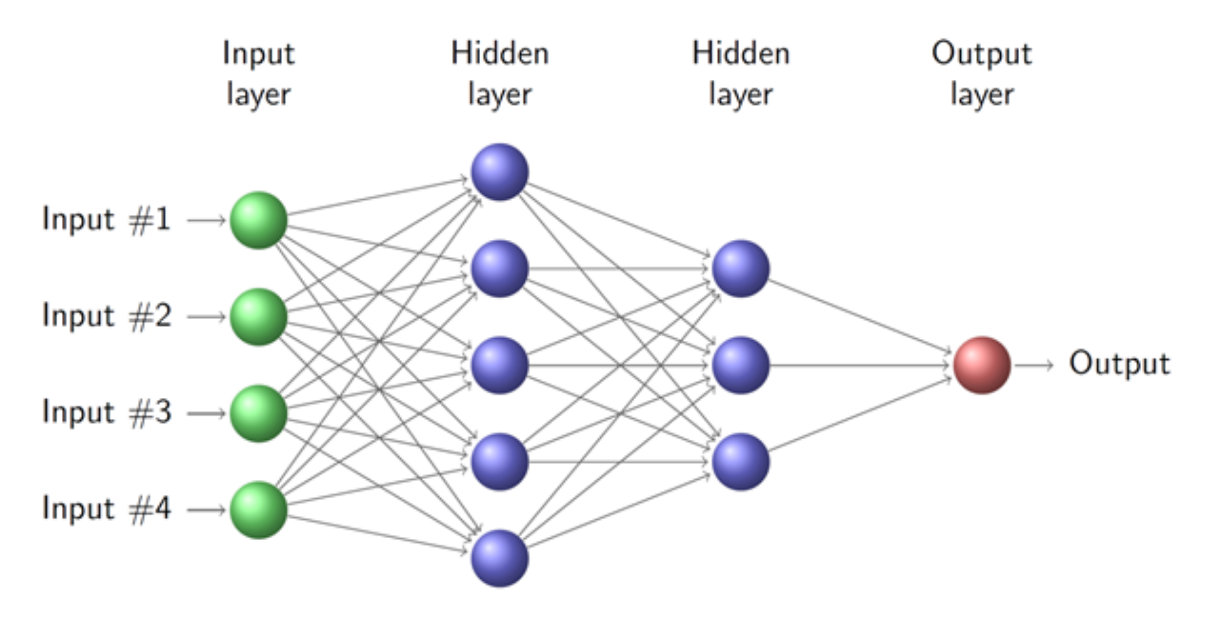
\includegraphics[scale=0.3]{ann.png}
\end{figure}
\end{frame}

\begin{frame}{Spiking Neural Network (SNN) Introduction}
\begin{itemize}
\item More closely resemble biological neural nets
\item Fire not during a propagation cycle, but when a specified `threshold membrane potential' crossed
\item A neuron's state is modeled by a differential equation that depends on input strength and as well as timing
\item More promise compared to other types of ANNs, but much more computationally intensive to both train and run
\item It is thought a primary advantage of SNNs comes from their ability to encode information in the frequency/rate of pulses and not just in their intensity, as with traditional networks
\end{itemize}
\end{frame}
%%%%%%%%%%%%%%%%%%%%%%%%%%%%%%%%%%%%%%%%%%%%%%%%%%%%%%%%%%%%%%%%%%%%%%%%%
%%%%%%%%%%%%%%%%%%%%%%%%%%%%%%%%%%%%%%%%%%%%%%%%%%%%%%%%%%%%%%%%%%%%%%%%%
% Section 2
\section{Biology of Hydra vulgaris}
%%%%%%%%%%%%%%%%%%%%%%%%%%%%%%%%%%%%%%%%%%%%%%%%%%%%%%%%%%%%%%%%%%%%%%%%%
%%%%%%%%%%%%%%%%%%%%%%%%%%%%%%%%%%%%%%%%%%%%%%%%%%%%%%%%%%%%%%%%%%%%%%%%%

\begin{frame}{Evolutionary History of H. vulgaris}
\begin{itemize}
\item \textit{Hydra} are small, freshwater hydrozoans (family Cnidaria)
\item Believed to have originated around 60 Mya
\item Cnidarians first appeared around 580 Mya, haven't changed much since
\item Very small repertoire of behaviors which is consistent across individuals and environments
\end{itemize}
\begin{figure}
\center
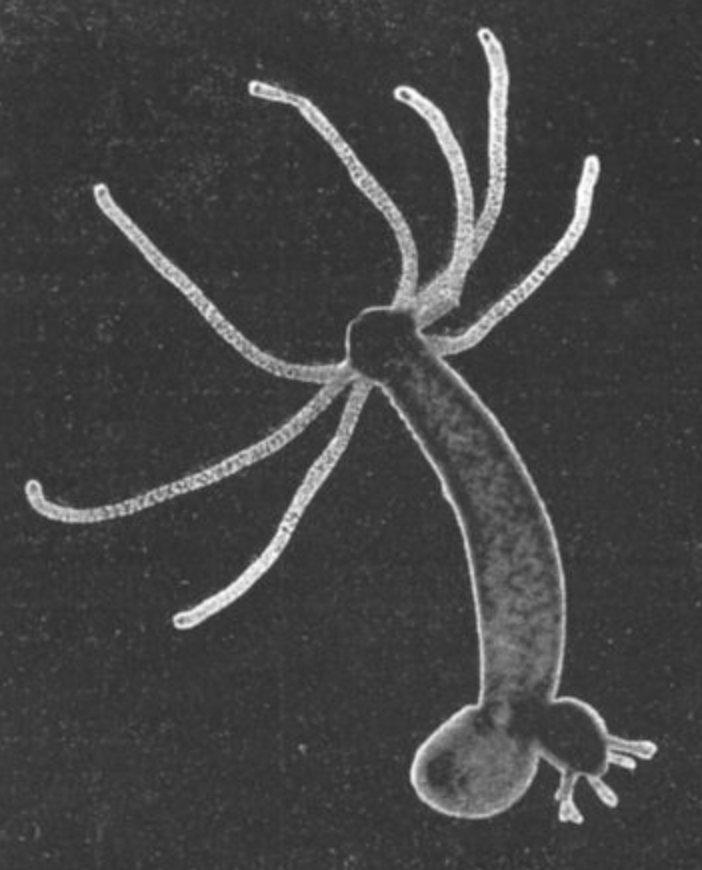
\includegraphics[scale=0.20]{hydra.png}
\end{figure}
\end{frame}

\begin{frame}{Nerve Nets}
\begin{itemize}
\item \textit{Hydra} have a diffuse nerve net rather than a CNS
\item Comprised of ganglia and a few types of sensory neurons
\item Once mature, a constant density gradient of neurons is maintained. Adults have no more than a few thousand neurons
\item Turns out nerve net is actually composed of non-overlapping circuits that correspond to specific sets of behaviors
\end{itemize}
\begin{figure}
\centering
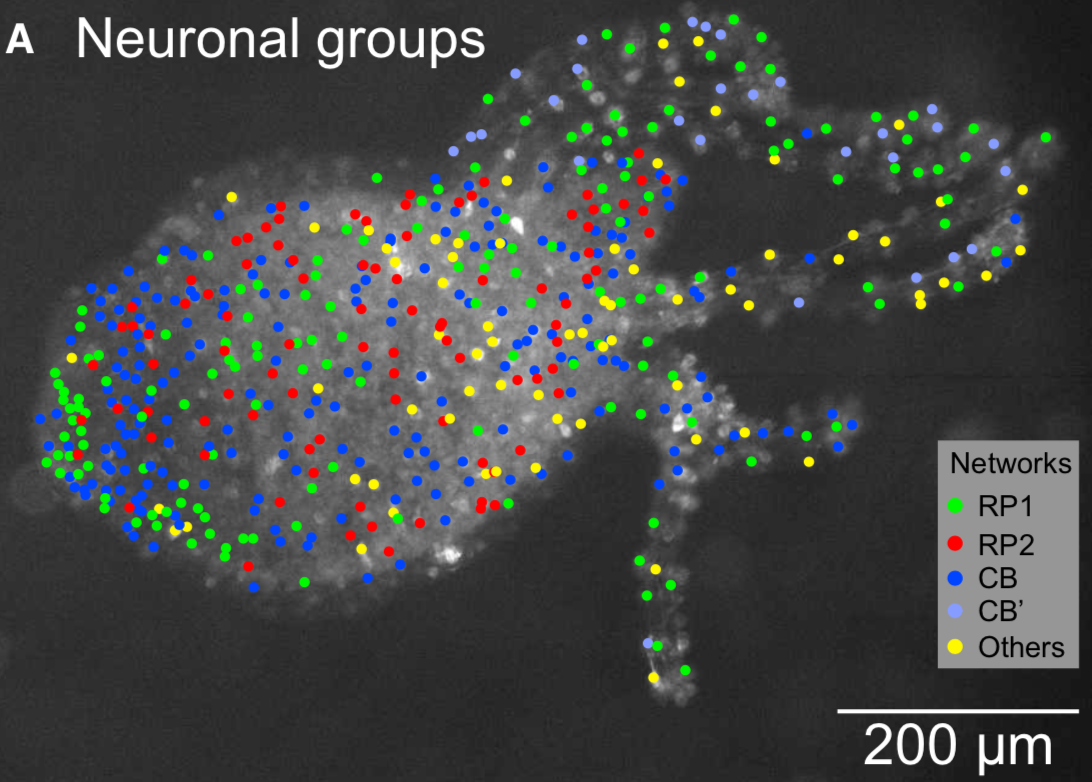
\includegraphics[scale=0.25]{hydra_map.png}
\end{figure}
\end{frame}

\begin{frame}{Separate Circuits}
\begin{itemize}
\item RP1 associated with longitudinal elongations
\item RP2 associated with radial contractions
\item CB associated with longitudinal contractions
\item STN associated with `nodding' behavior
\item RP1 and CB are antagonistic, no other interactions
\end{itemize}
\begin{figure}
\center
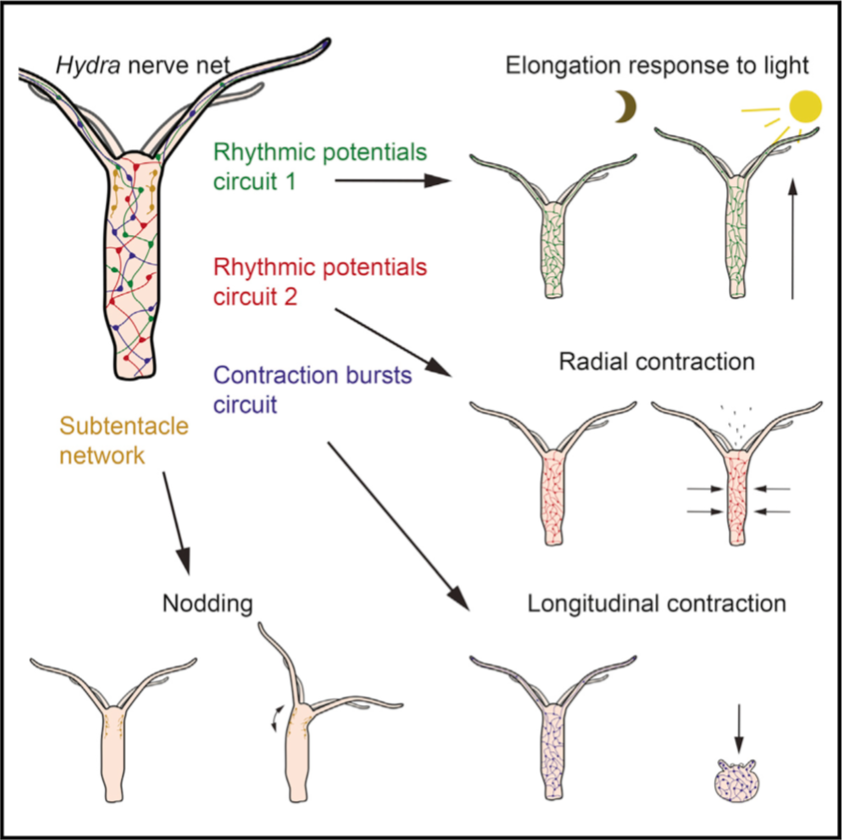
\includegraphics[scale=0.325]{hydra_movements.png}
\end{figure}
\end{frame}

\begin{frame}{Summary}
Advantages of \textit{Hydra} as a model organism:
\begin{itemize}
\item Very small size, so currents travel quickly and therefore the topology of the nerve net can be ignored at first approximation
\item Distinct behaviors appear to be controlled by distinct circuits, so analysis can be broken into many parts
\item Small amount of neurons and fixed neuronal density make simulation much easier
\end{itemize}
\end{frame}

%%%%%%%%%%%%%%%%%%%%%%%%%%%%%%%%%%%%%%%%%%%%%%%%%%%%%%%%%%%%%%%%%%%%%%%%%
%%%%%%%%%%%%%%%%%%%%%%%%%%%%%%%%%%%%%%%%%%%%%%%%%%%%%%%%%%%%%%%%%%%%%%%%%
% Section 3
\section{Network Framework}
%%%%%%%%%%%%%%%%%%%%%%%%%%%%%%%%%%%%%%%%%%%%%%%%%%%%%%%%%%%%%%%%%%%%%%%%%
%%%%%%%%%%%%%%%%%%%%%%%%%%%%%%%%%%%%%%%%%%%%%%%%%%%%%%%%%%%%%%%%%%%%%%%%%

\begin{frame}[fragile]{Neuron Model}
\begin{itemize}
\item Leaky integrate-and-fire (LIF) model:
\begin{equation*}
\frac{dV_{m}}{dt}=\frac{1}{C_{m}}\left(-\frac{(V_{m}-V_{m}^{eq})}{R_{m}}+I_{ext}\right)
\end{equation*}
\item Computationally simpler than Hodgkin-Huxley
\item Models neuron as RC circuit with leak term
\item Doesn't explicitly specify spiking behavior or refractory period, but easy to implement using iterative ODE methods
\item Possible implementation:
\begin{figure}
\begin{BVerbatim}[fontsize=\scriptsize]
if V(t+1) > threshold:
   V(t)   <- spike
   V(t+1) <- hyperpolarize
if t in refractory period:
   V(t+1) <- hyperpolarize
\end{BVerbatim}
\end{figure}
\end{itemize}
\end{frame}

\begin{frame}{Antagonistic Neural Circuits}
\begin{itemize}
\item Assume each neuron of RP1 emits an inhibitory neurotransmitter $E_{RP1}$ when spiking, and similarly for CB with $E_{CB}$. Using concentrations, the model is:
\begin{align*}
\frac{dV_{RP1}}{dt}&=\frac{1}{C_{RP1}}\left(-\frac{(V_{RP1}-V_{RP1}^{eq})}{R_{RP1}}+I_{ext}\left(1-E_{CB}\right)\right)\\
\frac{dV_{CB}}{dt}&=\frac{1}{C_{CB}}\left(-\frac{(V_{CB}-V_{CB}^{eq})}{R_{CB}}+I_{ext}\left(1-E_{RP1}\right)\right)\\
\frac{dE_{RP1}}{dt}&=d_{RP1}E_{RP1}\hspace{2em}\frac{dE_{CB}}{dt}=d_{CB}E_{CB}
\end{align*}
\end{itemize}
\end{frame}

\begin{frame}{Antagonistic Neural Circuits (cont.)}
\begin{figure}
\center
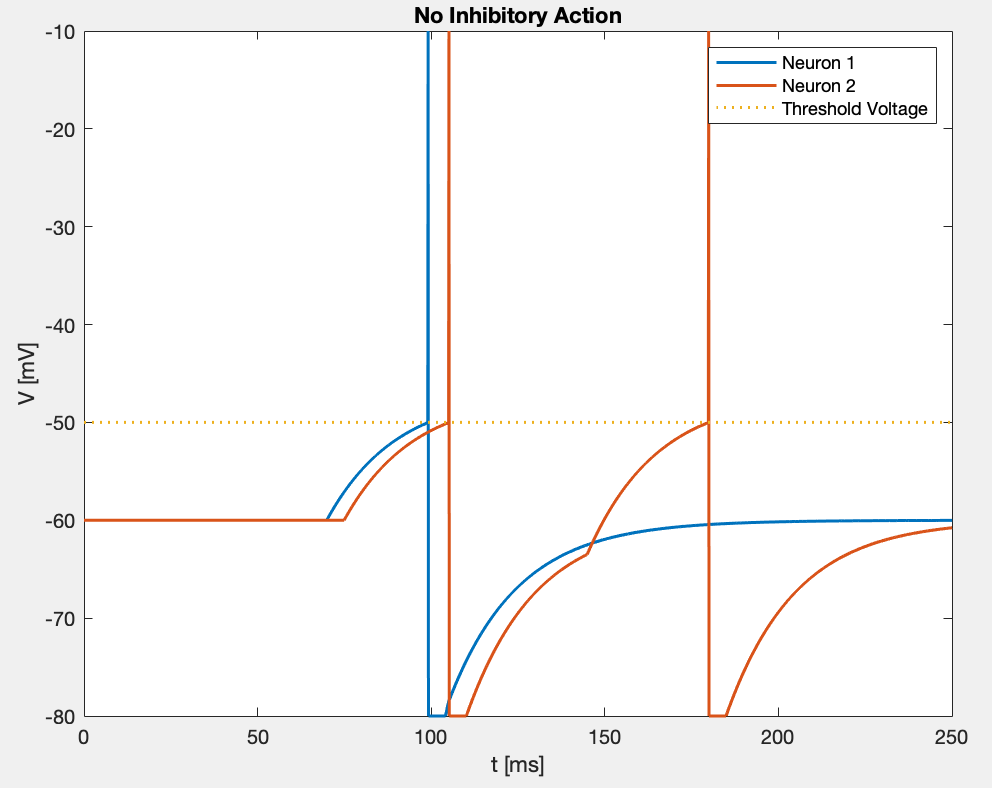
\includegraphics[scale=0.29]{no_inhib.png}\hspace{1em}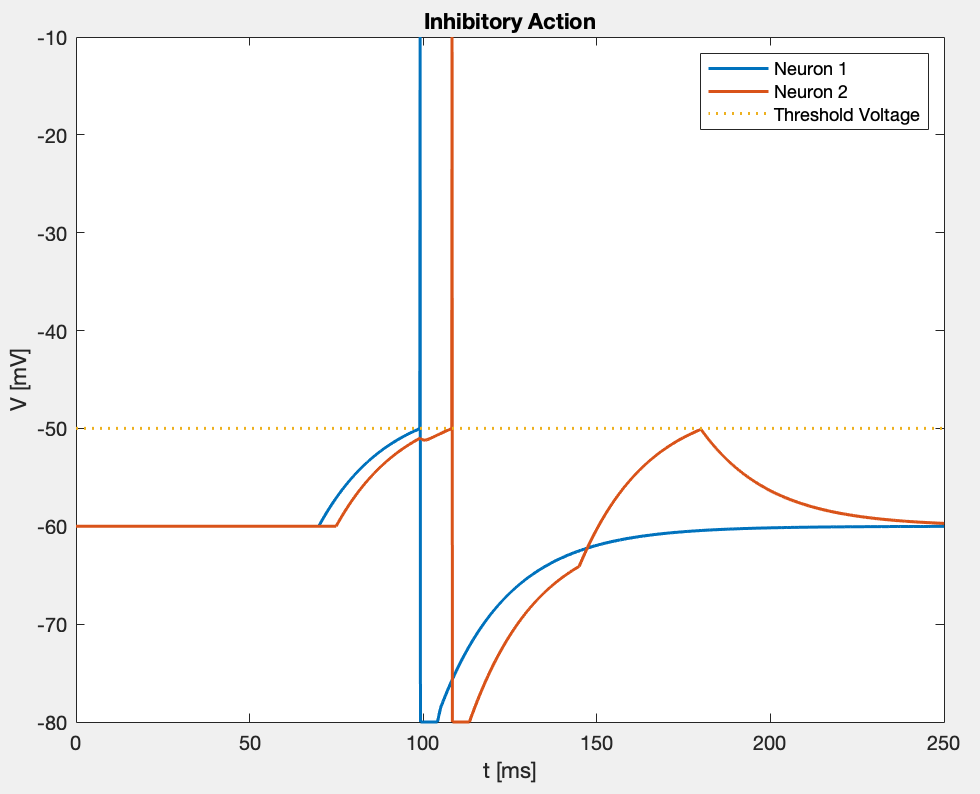
\includegraphics[scale=0.29]{inhib.png}
\caption{Simulation of two LIF neurons not acting on each other, and acting antagonistically, respectively. Input current is same in both simulations.}
\end{figure}
\end{frame}


%%%%%%%%%%%%%%%%%%%%%%%%%%%%%%%%%%%%%%%%%%%%%%%%%%%%%%%%%%%%%%%%%%%%%%%%%
%%%%%%%%%%%%%%%%%%%%%%%%%%%%%%%%%%%%%%%%%%%%%%%%%%%%%%%%%%%%%%%%%%%%%%%%%
% Section 4
\section{Optimizations}
%%%%%%%%%%%%%%%%%%%%%%%%%%%%%%%%%%%%%%%%%%%%%%%%%%%%%%%%%%%%%%%%%%%%%%%%%
%%%%%%%%%%%%%%%%%%%%%%%%%%%%%%%%%%%%%%%%%%%%%%%%%%%%%%%%%%%%%%%%%%%%%%%%%

\begin{frame}{SNN simplifications}
In our nerve network model, instead of fully simulating a continuous waveform for the state of the neuron, we keep track of the spikes at discrete timesteps instead. The primary advantage of spiked neural networks comes from the temporal coding, and this can be preserved with discrete timesteps.\newline\newline
One advantage of this approach is that the timestep size can be decreased if we find that information is not being encoded temporally as expected, or can be increased to save on processing power.
\end{frame}

\begin{frame}{Tensor Product Optimization}
We propose imposing non self-similar structure on the ``blank'' (before learning) nerve nets in the following fashion:\\
Where $H_1, H_2, \ldots, H_L$ are all graphs, we set  
$$ G = H_1 \otimes H_2 \otimes \cdots \otimes H_L $$
Where ``$\otimes$'' is the graph tensor product, equivalent to the matrix tensor product of the adjacency matrices of the graphs.\\
Tensor product $H \otimes K$ is equivalent to replacing every vertex in $H$ with a copy of $K$. Vertices have connections between them if their counterparts in either $H$ or $K$ have edges between them. This means a random walk on $H \otimes K$ can be simulated by a random walk on $H$ and $K$ at the same time.
\end{frame}

\begin{frame}{Tensor Product Optimization}
\begin{itemize}
    \item Note that the space required to store a graph as an adjacency matrix is $O(n^2)$ on the number of vertices
    \item If we assume $H_i$ has $n_i$ vertices, then we only require $ \sum_{i \in [1,L]} (n_i)^2 $ space to store the component graphs
    \item On the other hand, storing $G$ by itself requires space $ \prod_{i \in [1,L]} (n_i)^2 $
\end{itemize}
\end{frame}

\begin{frame}{Tensor Product Optimization, continued}
For large networks, the aforementioned size differences become very significant
\begin{itemize}
    \item Network with 5 layers of 100 neurons each will take only $5 \cdot 10^4$ units of memory to store by adjacency matrices
    \item the above 5-layer network describes a complex network with $100^{5}=10^{10}$ neurons that would take an adjacency matrix of size $10^{20}$ to describe
    \item assuming 1 byte memory per connection (very low estimate), the 5-layer network takes up about 50MB, while it's counterpart takes around a million TB to store directly. 
    \item Simulating and training this network is still computationally difficult, but space complexity  of is reduced
\end{itemize}
\end{frame}

\begin{frame}{Biological Motivation}
Making no assumptions about which genes affect the structure of the human brain, it is clearly impossible for the exact structure of the $>10^{10}$ neurons and $>10^{12}$ connections between them to be encoded in the mere $4 \cdot 10^{9}$ base pairs of the human genome. 

This tells us that there must be \textit{some} sort of repeated structure in most nerve networks. Granted, this repeated structure might not be in the form of graph tensor products,b

% However, some structure is clearly present even before any meaningful information is learned. Instead, some general structure may be encoded genetically, and the ``details'' are filled in as the organism develops.
\end{frame}

%%%%%%%%%%%%%%%%%%%%%%%%%%%%%%%%%%%%%%%%%%%%%%%%%%%%%%%%%%%%%%%%%%%%%%%%%
%%%%%%%%%%%%%%%%%%%%%%%%%%%%%%%%%%%%%%%%%%%%%%%%%%%%%%%%%%%%%%%%%%%%%%%%%
% Section 5
\section{Future Work}
%%%%%%%%%%%%%%%%%%%%%%%%%%%%%%%%%%%%%%%%%%%%%%%%%%%%%%%%%%%%%%%%%%%%%%%%%
%%%%%%%%%%%%%%%%%%%%%%%%%%%%%%%%%%%%%%%%%%%%%%%%%%%%%%%%%%%%%%%%%%%%%%%%%

\begin{frame}{Short term goals}
\begin{itemize}
    \item Using existing data in the literature, finish creating out model of the \textit{Hydra} antagonistic nerve nets
    \item After creating a network that exhibits temporal signalling behavior, we hope to find the largest timestep $\Delta t$ that preserves this behavior. Knowing the largest possible timestep lets us run simulations faster, and grants insights about the nature of the temporal signaling.
    \item Extend the tensor product optimization to allow replacement of vertices in $H_i$ with different graphs, not just $H_{i+1}$. This will in theory allow the representation of a wider variety of graph patterns, notably allowing differences in local structure between larger regions
\end{itemize}
\end{frame}

\begin{frame}{Long term future work}
\begin{itemize}
    \item Train the framework described here for \textit{Hydra} on actual behavioral data from specimens. With sufficient training, the network described should be able to, in more or less real time, predict the behavior of \textit{Hydra} in response to external stimuli.
    \item Chemical signalling in the human brain plays a far more complex role than the relatively simple antagonistic networks in \textit{Hydra}. Extending our model to the human brain is far outside the scope of this project or modern technology, but perhaps some insight into chemical signalling systems in nerve nets can be gained.
    \item With more information about the nature of the temporal signalling, it may be possible to model the frequency domain instead of the time domain. This would be both easier for a human to read, and less computationally expensive.
\end{itemize}
\end{frame}

%%%%%%%%%%%%%%%%%%%%%%%%%%%%%%%%%%%%%%%%%%%%%%%%%%%%%%%%%%%%%%%%%%%%%%%%%
%%%%%%%%%%%%%%%%%%%%%%%%%%%%%%%%%%%%%%%%%%%%%%%%%%%%%%%%%%%%%%%%%%%%%%%%
%%%%%%%%%%%%%%%%%%%%%%%%%%%%%%%%%%%%%%%%%%%%%%%%
\end{document}